\subsubsection{Généralités}
ipsec esp-sha1

\subsubsection{Mise en place côté serveur}

% TODO ecrire le noyau du routeur : c2800mn-advsecurityk9-mz.124-24.T.bin
\paragraph{Configuration de base}
~

Commençons par configurer les interfaces du routeur. L'interface connectée au réseau de l'ISIMA récupère son adresse IP via DHCP. Cela :
\begin{figure}[H]
	\begin{center}
		\begin{minipage}{0.90\textwidth}
			\begin{lstlisting}[frame=trBL]
(config)# hostname CISCOVPN
(config)# enable secret cisco
(config)# no ip domain-lookup
(config)# interface FastEthernet0/0
(config-if)# description interface to the external network
(config-if)# ip address dhcp
(config-if)# no shutdown
(config-if)# exit
(config)# interface FastEthernet0/1.1
(config-if)# description interface to the prof network
(config-if)# encapsulation dot1Q 333
(config-if)# ip address 10.0.0.1 255.255.255.0
(config-if)# exit
(config)# interface FastEthernet0/1.2
(config-if)# description interface to the student network
(config-if)# encapsulation dot1Q 111
(config-if)# ip address 192.168.0.1 255.255.255.0
(config-if)# exit
(config)# interface FastEthernet0/1
(config-if)# no shutdown
(config-if)# exit
			\end{lstlisting}
		\end{minipage}
	\end{center}
	\caption{Configuration des interfaces}
	\label{configuration_interfaces}
\end{figure}

~

Configurons maintenant les accès à distance au routeur :
\begin{figure}[H]
	\begin{center}
		\begin{minipage}{0.95\textwidth}
			\begin{lstlisting}[frame=trBL]
(config)# banner login #Unauthorized access prohibited - F5 only!#
(config)# banner motd #
This router is part of a wonderfull ZZ3F5 project for 2008-2009.
If you have any question, comment, insults, whatsoever...
please contact coscia@poste.isima.fr and dessaux@poste.isima.fr.
Thank you if you read this till the end.#
(config)# enable secret cisco
(config)# line con 0
(config-line)# logging synchronous
(config-line)# password cisco
(config-line)# login
(config-line)# exit
(config)# line vty 0 4
(config-line)# transport input telnet
(config-line)# password cisco
(config-line)# login
(config-line)# exit
(config)# service password-encryption
			\end{lstlisting}
		\end{minipage}
	\end{center}
	\caption{Configuration de l'accès à distance}
	\label{configuration_acces_a_distance}
\end{figure}

\paragraph{Configuration de l'authentification Radius}
~

Tout d'abord le serveur FreeRadius.
Authentication PAP entre radius server and cisco router :
Ajouter \verb|ciscovpn User-Password := "isima"|  au début du fichier \verb|/etc/raddb/users|, où ciscovpn est le hostname du routeur et isima le mot de passe qui lui sera associé.
Ajouter quelques lignes pour autoriser le router à interroger la base RADIUS dans le fichier /etc/raddb/clients.conf, et commenter la ligne shadow dans radiusd.conf

~


\begin{figure}[H]
	\begin{center}
		\begin{minipage}{0.90\textwidth}
			\begin{lstlisting}[frame=trBL]
(config)# aaa new-model
(config)# radius-server host 192.168.102.121 auth-port 1812
acct-port 1813 key isima
(config)# ip radius source-interface FastEthernet 0/0
(config)# aaa group server radius RadiusServer
(config-sg-radius)# radius-server host 192.168.102.121 auth-port
1812 acct-port 1813
(config-sg-radius)# exit
(config)# aaa authentication login default group RadiusServer
			\end{lstlisting}
		\end{minipage}
	\end{center}
	\caption{Configuration de l'authentification Radius}
	\label{configuration_authentification_radius}
\end{figure}


\paragraph{Configuration d'IPsec}
~

Les lignes qui suivent permettent de configurer la cryptographie isakmp :
\begin{itemize}
	\item algorithme de chiffrement triple DES.
	\item algorithme de hashage sha-1.
	\item authentification via clefs partagées.
	\item Diffie-Hellman 1024 bits.
	\item durée de vie du contexte cryptographique égale à une journée.
	\item utilisation du hostname plutôt que de l'adresse IP pour protéger les échanges.
\end{itemize}


\begin{figure}[H]
	\begin{center}
		\begin{minipage}{0.90\textwidth}
			\begin{lstlisting}[frame=trBL]
(config)# crypto isakmp policy 1
(config-isakmp)# encryption 3des
(config-isakmp)# hash sha
(config-isakmp)# authentication pre-share
(config-isakmp)# group 2
(config-isakmp)# lifetime 86400
(config-isakmp)# exit
(config)# crypto isakmp identity hostname
			\end{lstlisting}
		\end{minipage}
	\end{center}
	\caption{Configuration IKE}
	\label{configuration_ike}
\end{figure}

Ajoutons les pools DHCP qui fourniront leurs adresses IP aux étudiants et aux professeurs :
\begin{figure}[H]
	\begin{center}
		\begin{minipage}{0.90\textwidth}
			\begin{lstlisting}[frame=trBL]
(config)# ip local pool profs 10.0.1.20 10.0.1.254
(config)# crypto isakmp client configuration group profs
(config-isakmp-group)# key isimaprofs
(config-isakmp-group)# dns 10.0.0.11
(config-isakmp-group)# domain isima.fr
(config-isakmp-group)# pool profs
(config-isakmp-group)# exit

(config)# ip local pool students 192.168.1.20 192.168.1.254
(config)# crypto isakmp client configuration group students
(config-isakmp-group)# key isimastudents
(config-isakmp-group)# dns 192.168.1.11
(config-isakmp-group)# domain isima.fr
(config-isakmp-group)# pool students
(config-isakmp-group)# exit
			\end{lstlisting}
		\end{minipage}
	\end{center}
	\caption{Configuration des pools utilisateurs}
	\label{configuration_pools_utilisateurs}
\end{figure}


Configurons maintenant la police IPsec :
\begin{itemize}
	\item Mise en place de l'ACL pour indiquer que l'on veut filtrer l'ensemble du trafic IP.
	\item Encapsulation ESP, chiffrement 3des, intégrité sha-1.
	\item Mode tunnel (ie au niveau 3, par opposition au mode transport au niveau 4).
	\item Configuration de l'authentification des profs et des étudiants via le serveur radius.
\end{itemize}

\begin{figure}[H]
	\begin{center}
		\begin{minipage}{1\textwidth}
			\begin{lstlisting}[frame=trBL]
(config)# access-list 101 permit ip any any
(config)# crypto ipsec transform-set policy esp-3des esp-sha-hmac
(cfg-crypto-trans)# mode tunnel
(cfg-crypto-trans)# exit
(config)# crypto dynamic-map prof-map 1
(config-crypto-map)# set transform-set policy
(config-crypto-map)# exit

(config)# crypto map prof-map
(config)# crypto map prof-map 1 ipsec-isakmp dynamic prof-map
(config)# crypto map prof-map client authentication list RadiusServer
(config)# cryto map prof-map client configuration address respond
(config)# crypto map prof-map isakmp authorization list 101

(config)# aaa authorization network 101 local
			\end{lstlisting}
		\end{minipage}
	\end{center}
	\caption{Configuration de la police IPsec}
	\label{configuration_police_ipsec}
\end{figure}

La présence d'une seule crypto map et d'une identification en fonction du groupe dans le client peut provoquer des problème d'identification. En effet un étudiant peut facilement se faire passer pour un professeur et vice versa.
Pour remédier à ce problème, nous avons utiliser l'autorité de certification afin de pouvoir générer un certificat. Il est à noter que pour pouvoir effectuer cette manipulation, il faut au préalable installer sur le serveur Windows 2003 SCEP qui est un protocole dévélopper par CISCO pour enregistrer les certificats.
Lors de l'enregistrement du certificat sur le routeur, le processus va demander un mot de passe afin de bien vérifier l'identité du CA et du routeur. Ce mot de passe se trouve à l'adresse suivante : \verb|http://192.168.102.250/certsrv/mscep/mscep.dll|

Voici les différents phases pour enregistrer un certificat:


\begin{figure}[H]
	\begin{center}
		\begin{minipage}{1\textwidth}
			\begin{lstlisting}[frame=trBL]
(config)# crypto ca identity isima.fr
(ca-trustpoint)# enrollment url
http://192.168.102.250/certsrv/mscep/mscep.dll
(ca-trustpoint)# exit
(config)# crypto ca authenticate isima.fr
(config)# crypto ca trustpoint isima.fr
(ca-trustpoint)# crl optional
(ca-trustpoint)# exit
(config)# crypto isakmp policy 1
(config-isakmp)# authentication rsa-sig
(config-isakmp)# exit
			\end{lstlisting}
		\end{minipage}
	\end{center}
	\caption{Configuration de l'authentification via certificats}
	\label{configuration_authentification_certificats}
\end{figure}

Lorsque le routeur envoie sa requête l'autorité de certification, celui-ci à le pouvoir d'accepter ou de refuser sa requête. Dès que le CA à accepter le routeur, un message sur la console du routeur nous avertit que le certificat a été validé. En exécutant la commande \verb|show running-config| on trouve le certificat que le CA lui a attribué.


\subsubsection{Mise en place côté client}

La mise en place du côté client necessite l'installation du client CISCO sur sa machine. Ce client a la particularité d'être compatible avec Linux.

L'installation du client ne demande pas d'explication propre car celle-ci est relativement basique. Dans cette partie nous allons expliquer la configuration que le client doit faire lorsqu'il souhaite se connecter sur le serveur VPN.

Tout d'abord la création d'une nouvelle connexion se fait grâce au bouton ``NEW''. Une nouvelle fenêtre s'ouvre et demande à l'utilisateur de remplir différentes informations comme son groupe, l'adresse IP du serveur et la clé partagé. Ici dans notre exemple, on souhaite se connecter sur le réseau PROFS. La clé partagée est \verb isimaprofs.

\begin{figure}[H]
	\begin{center}
		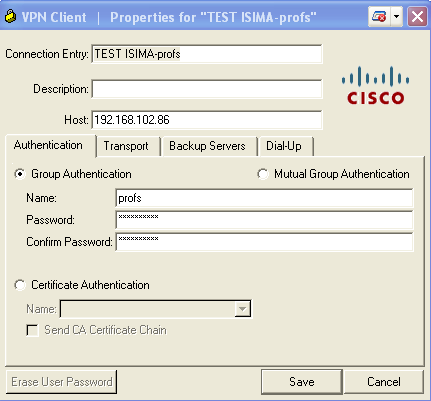
\includegraphics[width=0.75\textwidth]{partie_2/screen_windows/client_cisco.png}\\
	\end{center}
	\caption{Client CISCO}
	\label{VPN_CISCO}
\end{figure}


Une fois les informations remplie, le client va lancer la phase 1 d'ISAKMP afin de négocier la méthode d'authenrification avec le routeur CISCO. Si cette opération est réussite, une nouvelle fenêtre s'ouvre afin que l'utilisateur puisse entrer son login et son mot de passe et s'authentifier grâce au serveur NIS de l'ISIMA.

\begin{figure}[H]
	\begin{center}
		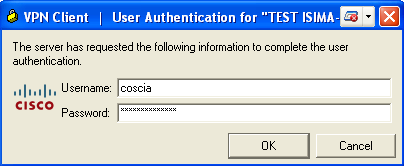
\includegraphics[width=0.75\textwidth]{partie_2/screen_windows/fenetre_connexion.PNG}\\
	\end{center}
	\caption{Identification du client}
	\label{VPN_CISCO_CLIENT}
\end{figure}



\subsubsection{Bilan et limites de la solution}

Dans cette partie, nous ferons des brefs tests de connexion afin de vérifier le bon fonctionnement de la solution.


\begin{figure}[H]
	\begin{center}
		\begin{minipage}{1\textwidth}
			\begin{lstlisting}[frame=trBL]


Configuration IP de Windows

Carte Ethernet Connexion au réseau local:

        Suffixe DNS propre à la connexion : isima.fr
        
	Adresse IP. . . . . . . . . . . . : 192.168.102.79
        
	Masque de sous-réseau . . . . . . : 255.255.255.0
        
	Passerelle par défaut . . . . . . : 192.168.102.60


Carte Ethernet Connexion au réseau local 3:

        Suffixe DNS propre à la connexion : isima.fr
       
	 Adresse IP. . . . . . . . . . .  : 10.0.1.22
        
	Masque de sous-réseau . . . . . . : 255.0.0.0
        
	Passerelle par défaut . . . . . . : 10.0.1.22


			\end{lstlisting}
		\end{minipage}
	\end{center}
	\caption{Adresse IP coté profs}
	\label{Adresse_IP_cote_profs}
\end{figure}


On peut refaire la même expérience en se connectant avec un utilisateur appartenant au groupe STUDENTS.

\begin{figure}[H]
	\begin{center}
		\begin{minipage}{1\textwidth}
			\begin{lstlisting}[frame=trBL]


Configuration IP de Windows

Carte Ethernet Connexion au réseau local:

        Suffixe DNS propre à la connexion : isima.fr
        
	Adresse IP. . . . . . . . . . . . : 192.168.102.79
        
	Masque de sous-réseau . . . . . . : 255.255.255.0
        
	Passerelle par défaut . . . . . . : 192.168.102.60


Carte Ethernet Connexion au réseau local 3:

        Suffixe DNS propre à la connexion : isima.fr
       
	 Adresse IP. . . . . . . . . . .  : 192.168.1.20
        
	Masque de sous-réseau . . . . . . : 255.255.255.0
        
	Passerelle par défaut . . . . . . : 192.168.1.20

\end{lstlisting}
		\end{minipage}
	\end{center}
	\caption{Adresse IP coté eleve}
	\label{Adresse_IP_cote_eleve}
\end{figure}

On remarque bien que la solution CISCO est fonctionnelle, en fonction du groupe d'appartenance le routeur est capable de rediriger l'utilisateur sur le bon réseau.

D'un point de vue sécurité, la solution CISCO est très performante. En effet, une fois le tunnel VPN crée toutes les informations sont cryptées y compris le login de l'utilisateur. Cependant, le fait de remplir dans le client VPN le groupe d'appartenance ainsi que la clé ne nous permet pas de réellement identifer l'utilisateur. Imaginons qu'un élève connaisse la clé PROFS, il pourra sans aucun problème se connecter avec son mot de passe tradionnel sur le réseau professeur. Afin d'éviter ce problème, la solution serait de mettre en place un système de certificat en utilisant l'autorité de certification installée sur le serveur Windows 2003. Nous avons réussi à fournir un certificat au routeur CISCO et à l'intégrer dans sa configuration. Du point de vue client, nous avons été capable d'en générer un. Par contre, en tant qu'utilisateur nous n'avons pas réussi à monter le VPN. Nous pensons que le problème provient du type de certificat créé.